\documentclass[11pt]{article}
\usepackage[left=0.2in,right=0.2in,top=0.9in,bottom=0.9in]{geometry}
\usepackage{amsmath}
\usepackage{microtype}
\usepackage{xcolor}
\usepackage{titlesec}
\usepackage{enumitem}
\usepackage{multicol}
\usepackage{lettrine}
\usepackage{fancyhdr}
\usepackage{mathpazo}
\usepackage{setspace}
\usepackage{ragged2e}
\usepackage{tcolorbox}
\usepackage{pgfplots}
\usepackage[hidelinks]{hyperref}

\setlength{\parindent}{0pt}
\setlength{\parskip}{0.55\baselineskip}
\definecolor{duskblue}{HTML}{2E5077}
\definecolor{amberglow}{HTML}{FFA630}
\definecolor{crimsonviolet}{HTML}{611C35}
\definecolor{pacificblue}{HTML}{4DA1A9}

\setstretch{1.06}
\setlength{\columnsep}{20pt}
\setlength{\columnseprule}{0.2pt}
\def\columnseprulecolor{\color{pacificblue}}
\emergencystretch=1.4em

\setlength{\headheight}{22pt}

\pagestyle{fancy}
\fancyhf{}
\fancyhead[L]{\small\textcolor{amberglow}{\textbf{SCIENCE \& WORK}}}
\fancyhead[C]{\small\textcolor{crimsonviolet}{Physics \& Career Special}}
\fancyhead[R]{\small{March 2026}}
\fancyfoot[L]{\small\textcolor{crimsonviolet}{Magazine Feature}}
\fancyfoot[C]{\small\textcolor{crimsonviolet}{\thepage}}
\fancyfoot[R]{\small\textcolor{amberglow}{www.matthewd0yle.com}}
\renewcommand{\headrulewidth}{0.4pt}
\renewcommand{\footrulewidth}{0.4pt}
\renewcommand{\headrule}{\hbox to\headwidth{\leaders\hrule height \headrulewidth\hfill}}
\renewcommand{\footrule}{\hbox to\headwidth{\leaders\hrule height \footrulewidth\hfill}}

\tcbset{
  colback=amberglow!12,
  colframe=crimsonviolet,
  arc=0pt,
  left=0.9em,
  right=0.9em,
  top=0.65em,
  bottom=0.65em,
  boxrule=0.8pt
}

\titleformat{\section}{\large\bfseries\color{duskblue}}{}{0em}{}
\titlespacing*{\section}{0pt}{1.2\baselineskip}{0.45\baselineskip}
\titleformat{\subsection}{\normalsize\bfseries\color{duskblue}}{}{0em}{}
\titlespacing*{\subsection}{0pt}{0.9\baselineskip}{0.2\baselineskip}
\newcommand{\rcite}[1]{\textsuperscript{[#1]}}
\pgfplotsset{compat=1.18}

\begin{document}

\vspace*{0.35em}
{\fontsize{22}{25}\selectfont\textbf{Why Learning Physics Deeply Changes a Career}}\par\vspace{0.35em}
{\large\textcolor{crimsonviolet}{How advanced physics training quietly builds the kind of mind that thrives in modern work}}\par\vspace{0.95em}

\begin{tcolorbox}
\textbf{At a glance:} High-level physics education strengthens model-building, quantitative judgment, and decision quality---skills that compound into faster trust, broader mobility, and long-term career resilience.
\end{tcolorbox}

\vspace{0.6em}

\begin{multicols}{2}
\RaggedRight

\lettrine[lines=3,loversize=0.08,findent=2pt,nindent=0pt]{M}{ost} people think of physics as equations, lab reports, and difficult exams. But at a high level, physics is really training in a rare way of thinking: precise, creative, and relentlessly honest about what is true.

That way of thinking does not stay in the classroom. It follows people into startups, hospitals, policy teams, finance desks, engineering firms, classrooms, and executive offices. In many careers, the strongest advantage is not knowing one formula. It is knowing how to approach complex problems under uncertainty. High-level physics builds exactly that.\rcite{1,3}

\section*{What Physics Really Teaches}

Advanced physics education develops a set of professional ``superpowers'' that transfer across industries:

\begin{itemize}[leftmargin=1.5em]
  \item \textbf{Model building:} turning messy reality into useful, testable structures.
  \item \textbf{Quantitative judgment:} estimating scale, risk, and feasibility before others can.
  \item \textbf{Causal reasoning:} separating correlation from mechanism.
  \item \textbf{Error discipline:} checking assumptions, limits, and hidden failure modes.
  \item \textbf{Intellectual resilience:} staying calm through ambiguity and hard iteration.
\end{itemize}

These abilities are not cosmetic. They directly influence hiring, promotion, and leadership outcomes.\rcite{2,4}

\section*{Career Effects in the Real World}

\subsection*{Snapshot from recent outcomes data}
The latest AIP outcomes survey shows that most new physics bachelors quickly enter high-value paths: 53\% took potentially permanent employment and 35\% entered graduate or professional school.\rcite{1}

\begin{center}
\begin{tikzpicture}
\begin{axis}[
    ybar,
    width=.8\linewidth,
    height=0.28\textheight,
    ymin=0,
    ymax=60,
    bar width=9pt,
    ylabel={Percent of new physics bachelors},
    symbolic x coords={Potentially permanent employment,Graduate/professional school,Postdoc temp appointment,Other temporary position,Seeking employment,Other},
    xtick=data,
    x tick label style={rotate=35,anchor=east,font=\scriptsize},
    ymajorgrids=true,
    grid style={pacificblue!45},
    nodes near coords,
    every node near coord/.append style={font=\scriptsize},
    enlarge x limits=0.08,
]
\addplot[fill=amberglow!85,draw=crimsonviolet] coordinates {
  (Potentially permanent employment,53)
  (Graduate/professional school,35)
  (Postdoc temp appointment,2)
  (Other temporary position,7)
  (Seeking employment,2)
  (Other,2)
};
\end{axis}
\end{tikzpicture}
\end{center}

{\footnotesize\textit{Data source: AIP Statistical Research Center, academic years 2022--23 and 2023--24.}\rcite{1}}

\subsection*{1. Faster trust from technical teams}
People with deep physics training often communicate in a way engineers and scientists trust: clear assumptions, explicit trade-offs, and quantitative backing. That trust shortens the path to influence.\rcite{2,4}

\subsection*{2. Better performance in high-uncertainty roles}
Many modern jobs involve incomplete data and moving targets. Physics-trained professionals are used to working from first principles, so they can make progress when playbooks fail.\rcite{2,5}

\subsection*{3. Strong mobility across sectors}
Because the core skill is structured thinking, not one narrow tool, physics learners can pivot more easily: research to product, academia to industry, engineering to strategy, or technical work to entrepreneurship.\rcite{1,3,6}

\subsection*{4. Distinctive leadership style}
At senior levels, success depends on decision quality. Leaders with physics backgrounds often excel at framing problems, stress-testing plans, and asking the one question that reveals hidden risk.\rcite{2,4}

\section*{The Economic and Professional Payoff}

Career success is multidimensional: income, autonomy, impact, and durability over time. High-level physics study tends to improve all four through a compounding mechanism:

\begin{center}
\footnotesize\textit{Deep reasoning + technical credibility + adaptability $\Rightarrow$ accelerating opportunity}
\end{center}

Early in a career, the benefit may look modest---better analysis, stronger interviews, cleaner execution. Over a decade, it compounds into larger responsibilities, broader options, and more strategic roles.\rcite{1,2,4}

\section*{A Human Effect Beyond Career}

There is also a personal transformation. Serious physics study teaches humility before evidence and confidence in method. You learn that confusion is not failure; it is the start of understanding. That mindset makes people better learners for life, and lifelong learners are the ones who remain valuable as industries change.\rcite{5}

\section*{Bottom Line}

Learning physics to a high level does not guarantee one specific job title. It does something more powerful: it equips a person with a portable, future-proof way to think.

In a world where tools, markets, and technologies shift constantly, that may be one of the strongest foundations for lasting career success.\rcite{1,2,4}

\end{multicols}

\section*{References}
\begingroup
\small
\begin{enumerate}[leftmargin=1.4em,itemsep=0.35em]
  \item American Institute of Physics Statistical Research Center. \textit{Initial Employment Sectors of New Physics Bachelors, Academic Years 2022--23 and 2023--24} (January 14, 2026). Available: \href{https://www.aip.org/statistics/initial-employment-sectors-of-new-physics-bachelors-academic-years-2022-23-and-2023-24}{AIP Statistical Research Center}.
  \item Mulvey, P., \& Pold, J. \textit{Physics Bachelors Initial Employment Booklet -- Academic Years 2020--21 and 2021--22}. AIP Statistical Research Center (January 8, 2025). DOI: \url{https://doi.org/10.1063/sr.aa204240a3}
  \item American Institute of Physics Statistical Research Center. \textit{Field of Employment for New Physics Bachelors, Academic Years 2020--21 and 2021--22} (January 10, 2025). Available: \href{https://www.aip.org/statistics/field-of-employment-for-new-physics-bachelors-academic-years-2020-21-and-2021-22}{AIP Statistical Research Center}.
  \item Deming, D. J. \textit{The Growing Importance of Social Skills in the Labor Market}. \textit{Quarterly Journal of Economics} 132(4), 1593--1640 (2017). DOI: \url{https://doi.org/10.1093/qje/qjx022}
  \item National Academies of Sciences, Engineering, and Medicine. \textit{How People Learn II: Learners, Contexts, and Cultures}. National Academies Press (2018). DOI: \url{https://doi.org/10.17226/24783}
  \item American Physical Society. \textit{Careers Guide 2025: A Guide to Careers in Physics}. \url{https://www.aps.org/publications/reports/careers-guide}
\end{enumerate}
\endgroup

\end{document}